%%%%%%%%%%%%%%%%%%%%%%%%%%%%%%%%%%%%%%%%%
% a0poster Portrait Poster
% LaTeX Template
% Version 1.0 (22/06/13)
%
% The a0poster class was created by:
% Gerlinde Kettl and Matthias Weiser (tex@kettl.de)
% 
% This template has been downloaded from:
% http://www.LaTeXTemplates.com
%
% License:
% CC BY-NC-SA 3.0 (http://creativecommons.org/licenses/by-nc-sa/3.0/)
%
%%%%%%%%%%%%%%%%%%%%%%%%%%%%%%%%%%%%%%%%%

%----------------------------------------------------------------------------------------
%	PACKAGES AND OTHER DOCUMENT CONFIGURATIONS
%----------------------------------------------------------------------------------------

\documentclass[a0,landscape]{a0poster}

\usepackage{multicol} % This is so we can have multiple columns of text side-by-side
\columnsep=50pt % This is the amount of white space between the columns in the poster
\columnseprule=3pt % This is the thickness of the black line between the columns in the poster

\usepackage[svgnames]{xcolor} % Specify colors by their 'svgnames', for a full list of all colors available see here: http://www.latextemplates.com/svgnames-colors

\usepackage{times} % Use the times font
%\usepackage{palatino} % Uncomment to use the Palatino font
\usepackage{array}
\usepackage{float}
\usepackage{hyperref}
\hypersetup{
	colorlinks = true, %Colours links instead of ugly boxes
	urlcolor = blue, %Colour for external hyperlinks
	linkcolor = red, %Colour of internal links
	citecolor = red %Colour of citations
}
\usepackage{graphicx} % Required for including images
%\graphicspath{{/home/vibishan/Dropbox/cancer work/regression analysis/TeX files}} % Location of the graphics files
\usepackage{booktabs} % Top and bottom rules for table\textsl{}
\usepackage[font=small,labelfont=bf]{caption} % Required for specifying captions to tables and figures
\usepackage{amsfonts, amsmath, amsthm, amssymb} % For math fonts, symbols and environments
\usepackage{wrapfig} % Allows wrapping text around tables and figures
\usepackage{pgf}
\usepackage[backend=biber, style=numeric-comp, citestyle=science, doi=false, isbn=false, url=false, eprint=false]{biblatex}
\addbibresource{poster.bib}

\begin{document}

%----------------------------------------------------------------------------------------
%	POSTER HEADER 
%----------------------------------------------------------------------------------------

% The header is divided into two boxes:
% The first is 75% wide and houses the title, subtitle, names, university/organization and contact information
% The second is 25% wide and houses a logo for your university/organization or a photo of you
% The widths of these boxes can be easily edited to accommodate your content as you see fit
\begin{minipage}[l]{0.95\linewidth}
	{ \color{NavyBlue} {\fontsize{100}{120}\selectfont Context-dependent selection as the keystone in somatic evolution of cancer}}\\[1.5cm] % Title
	%\textit{Linear vs saturation relationships}\\[2cm] % Subtitle
	{\huge \textbf{Vibishan B and Milind G. Watve}}\\[1cm] % Author(s)
	{\LARGE Department of Biology, Indian Institute of Science Education and Research (IISER), Pune}\\[0.4cm] % University/organization
	{\LARGE Corresponding author: {\color{Red}\underline{milind@iiserpune.ac.in}}}
\end{minipage}
\begin{minipage}[r]{0.05\linewidth}
	
\includegraphics[width=\linewidth]{logo.png}
\end{minipage}

\color{NavyBlue} % SaddleBrown color for the introduction
\large
\section*{Abstract}
	Somatic evolution of cancer involves a series of mutations, and attendant changes, in one or more clones of cells. Unlike a ``bad luck'' type model, the notion of clonal expansion adds competition-driven selection to the supposedly random process of somatic mutagenesis, with the implicit assumption that any mutation leading to partial loss of regulation of cell proliferation will give a selective advantage to the mutant. However, a number of experiments show that an intermediate pre-cancer mutant has only a conditional selective advantage; given that tissue microenvironmental conditions differ across individual organisms, this selective advantage to a mutant should be widely distributed over the population of organisms. We evaluate three models, namely ``bad luck'', context-independent, and -dependent selection, in a comparative framework, on their ability to predict patterns in total incidence, age-specific incidence, and their ability to explain Peto’s paradox. Results show that context dependence is necessary and sufficient to explain observed epidemiological patterns, and that cancer incidence is largely selection-limited, as opposed to the mutation-centric, ``bad luck'' view. A wide range of physiological, genetic and behavioural factors influence the tissue micro-environment, and could therefore be the source of this context dependence in somatic evolution of cancer. The identification and targeting of these micro-environmental factors that influence the dynamics of selection offer new possibilities for cancer prevention. Our work also seeks to renew interest in the comparative evaluation framework, whose application has seen a lull in cancer literature, despite the possibilities of rejection it offers for potential theories of carcinogenesis.
%\vspace{1cm} % A bit of extra whitespace between the header and poster content
\begin{multicols}{3}
	%----------------------------------------------------------------------------------------
	
	%\begin{multicols}{3} % This is how many columns your poster will be broken into, a portrait poster is generally split into 2 columns
	
	%%----------------------------------------------------------------------------------------
	%%	ABSTRACT
	%%----------------------------------------------------------------------------------------
	%
	%\color{Navy} % Navy color for the abstract
	%
	%\begin{abstract}
	%
	%Sed fringilla tempus hendrerit. Vestibulum ante ipsum primis in faucibus orci luctus et ultrices posuere cubilia Curae; Etiam ut elit sit amet metus lobortis consequat sit amet in libero. Lorem ipsum dolor sit amet, consectetur adipiscing elit. Phasellus vel sem magna. Nunc at convallis urna. isus ante. Pellentesque condimentum dui. Etiam sagittis purus non tellus tempor volutpat. Donec et dui non massa tristique adipiscing. Quisque vestibulum eros eu. Phasellus imperdiet, tortor vitae congue bibendum, felis enim sagittis lorem, et volutpat ante orci sagittis mi. Morbi rutrum laoreet semper. Morbi accumsan enim nec tortor consectetur non commodo nisi sollicitudin. Proin sollicitudin. Pellentesque eget orci eros. Fusce ultricies, tellus et pellentesque fringilla, ante massa luctus libero, quis tristique purus urna nec nibh.
	%
	%\end{abstract}
	
	%----------------------------------------------------------------------------------------
	%	INTRODUCTION
	%----------------------------------------------------------------------------------------
	
	\color{black}
	\large
	
		\section{Epidemiological observations}
		\begin{minipage}{.5\linewidth}
		\flushleft
			\begin{figure}[H]
				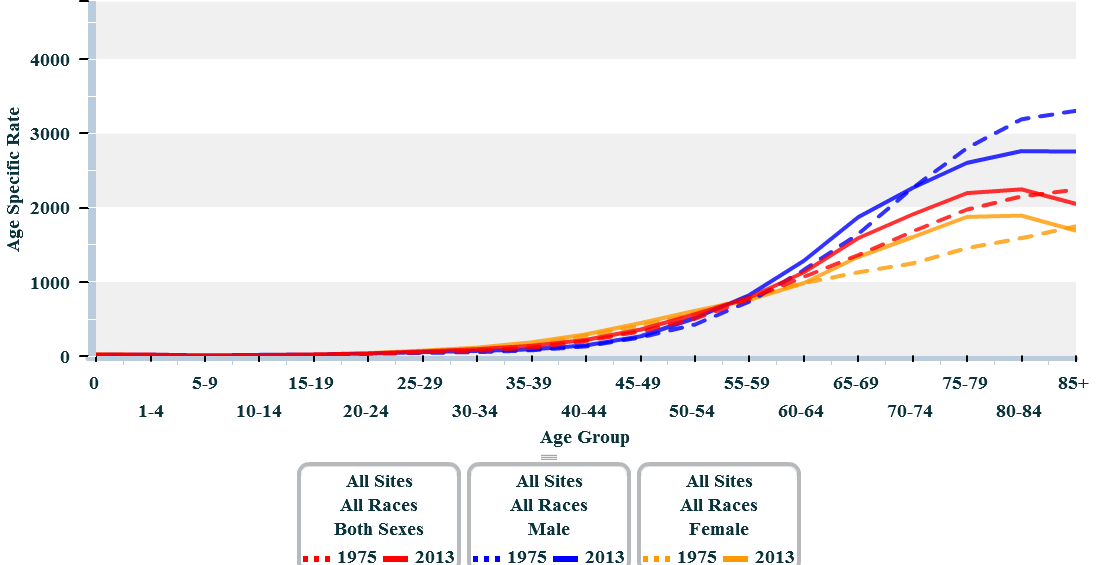
\includegraphics[width=\linewidth]{fig1.png}
				\caption{Cancer incidence vs age, from SEER9 \cite{AmericanCancerSociety2016}}
			\end{figure}
		\end{minipage}
		\hspace{0.05\linewidth}
		\begin{minipage}{.5\linewidth}
		\flushright
				\begin{itemize}
					\item Late-life decline with age
					\item Cancer risk saturates with $n$
					\item Non-mutagenic carcinogens
					\item \textbf{Peto's paradox}
				\end{itemize}
		\end{minipage}
		
		\section{``Bad luck'' model}
		\begin{minipage}{.25\linewidth}
		% {\small
		Equations used:
		\begin{itemize}
			\item $p_{can}=1-(1-p)^{n}$
			\item $p_{A}=1-(1-p_{can})^A$
		\end{itemize}
		\end{minipage}
		\hspace{0.03\linewidth}
		\begin{minipage}{.65\linewidth}
			\begin{figure}[H]
				\flushright
				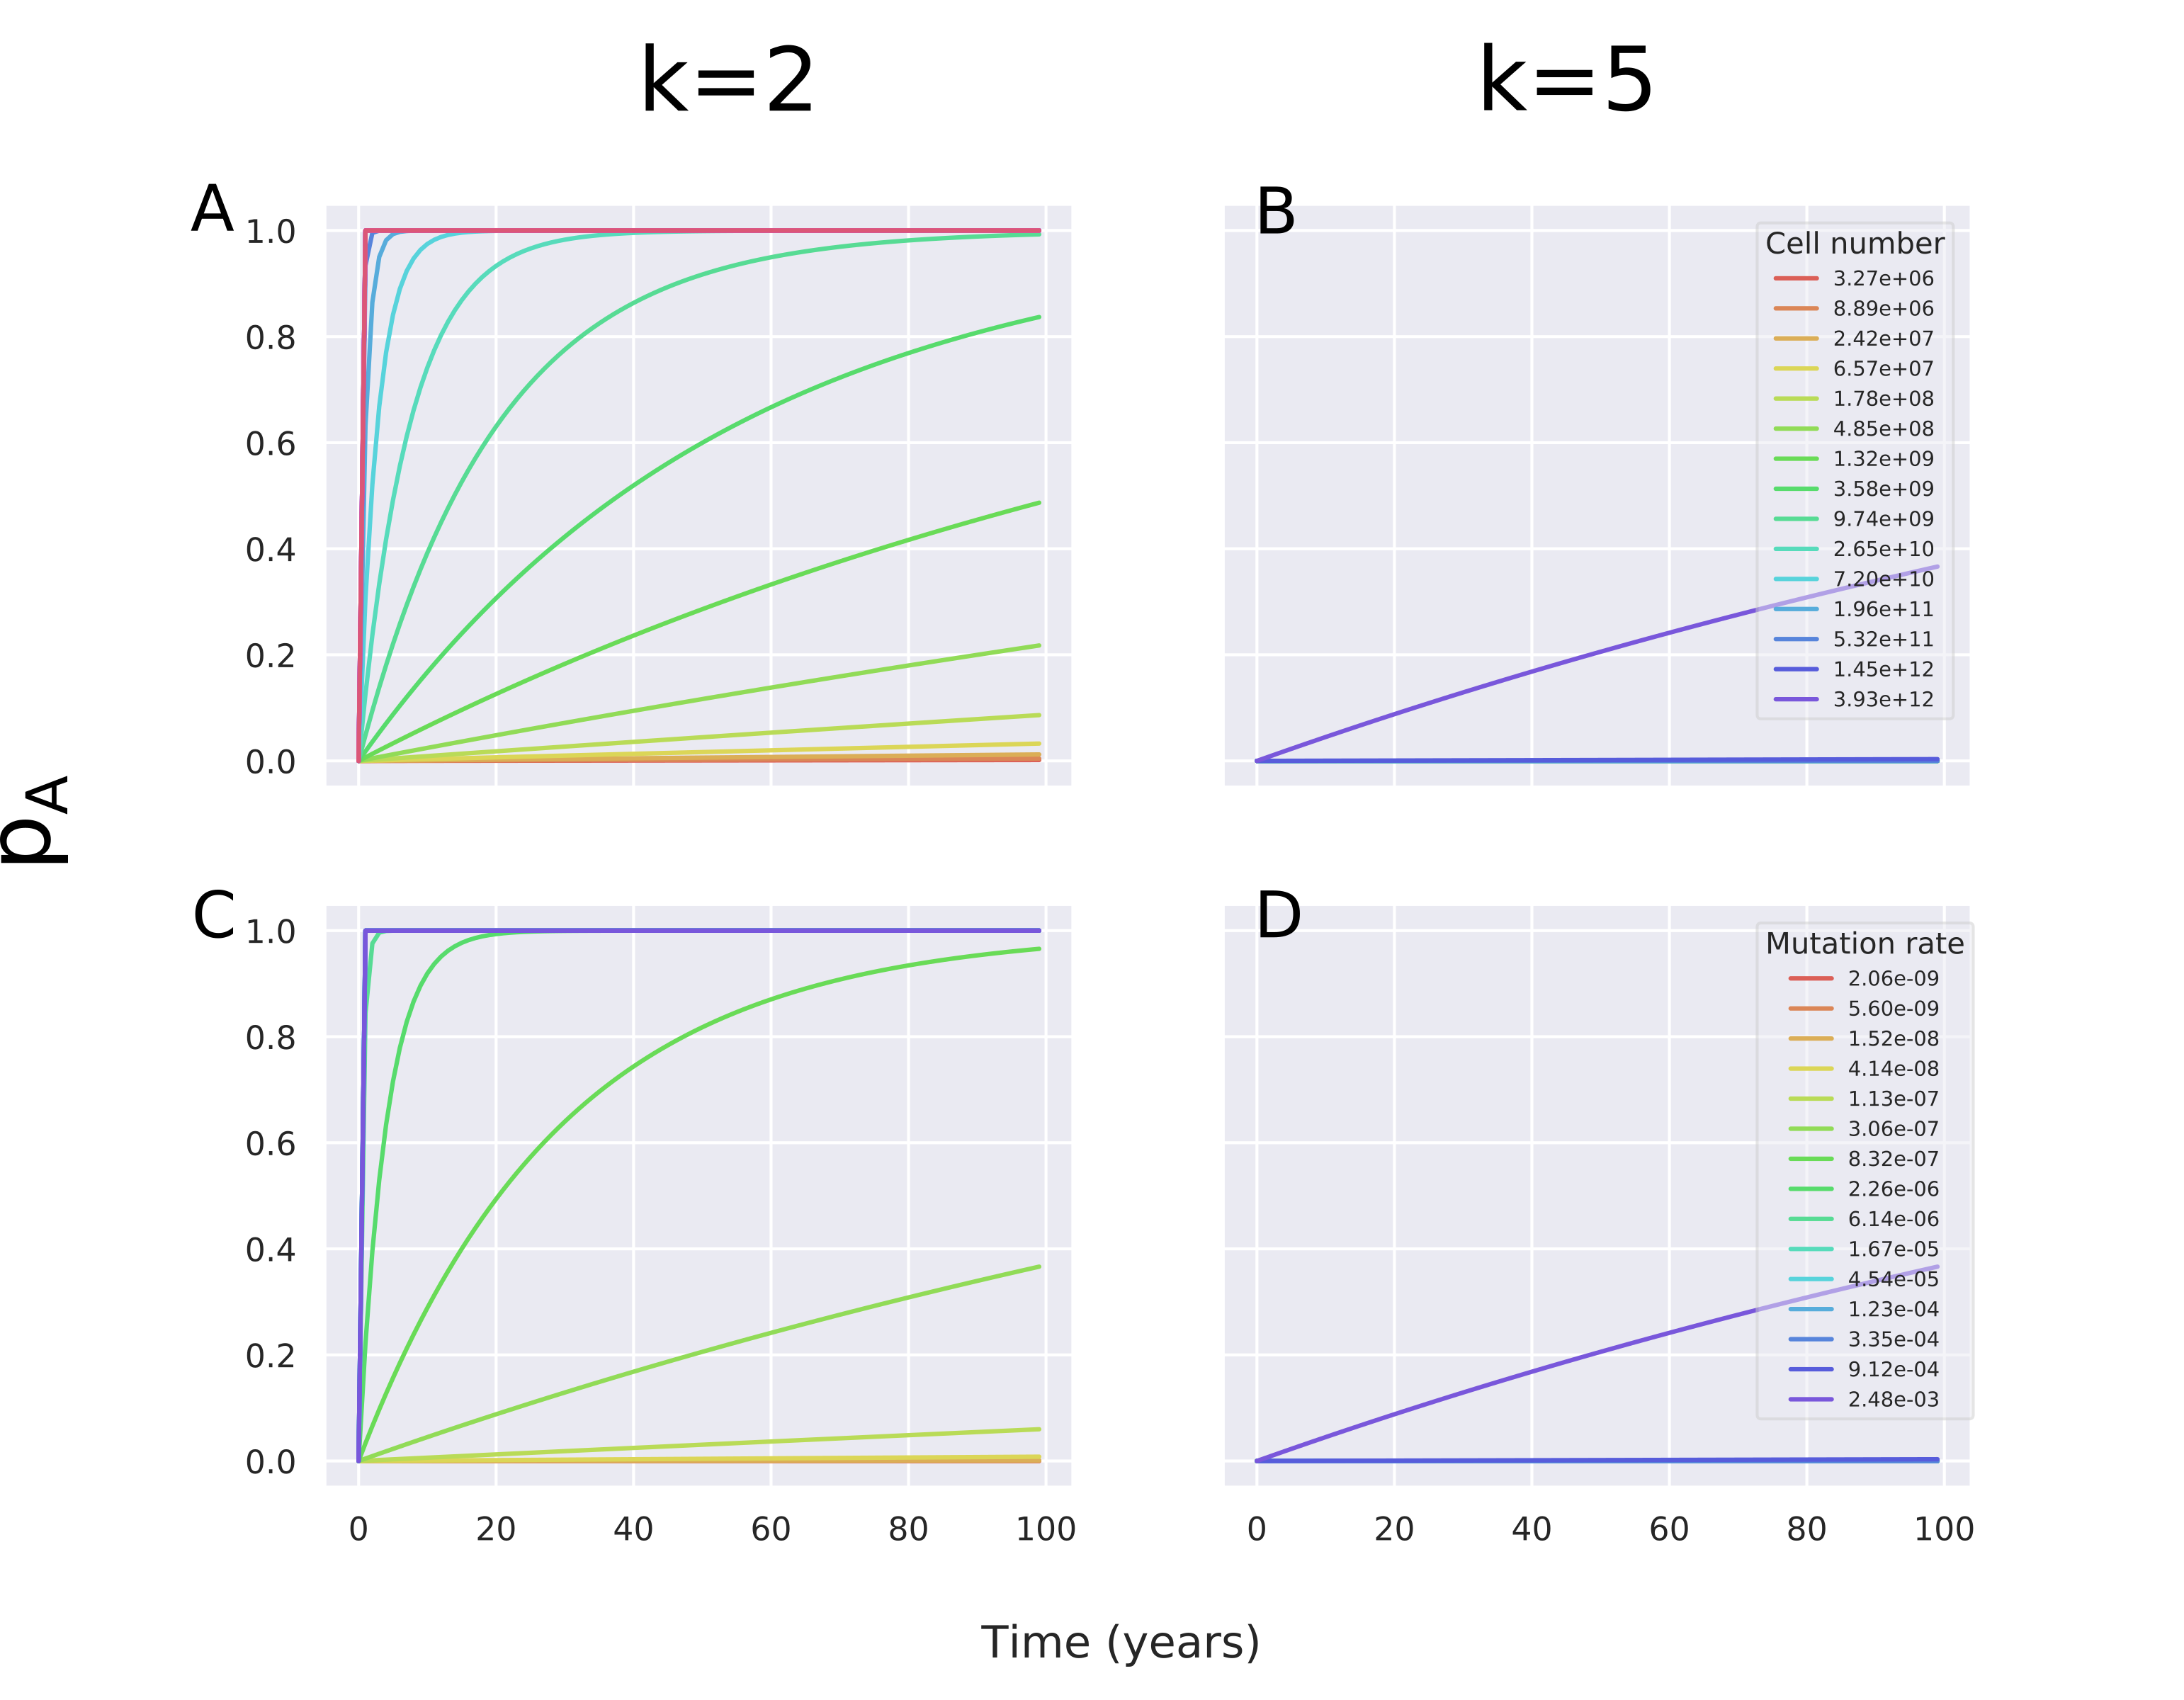
\includegraphics[width=\linewidth]{fig2.png}
				\caption{Incidence vs age, with $n$ and $p$}
			\end{figure}
		\end{minipage}


		\begin{minipage}{\linewidth}
		\begin{figure}[H]
			%		\def\svgwidth{0.25\columnwidth}
			%		\input{r_elimination.pdf_tex}
			\flushright
			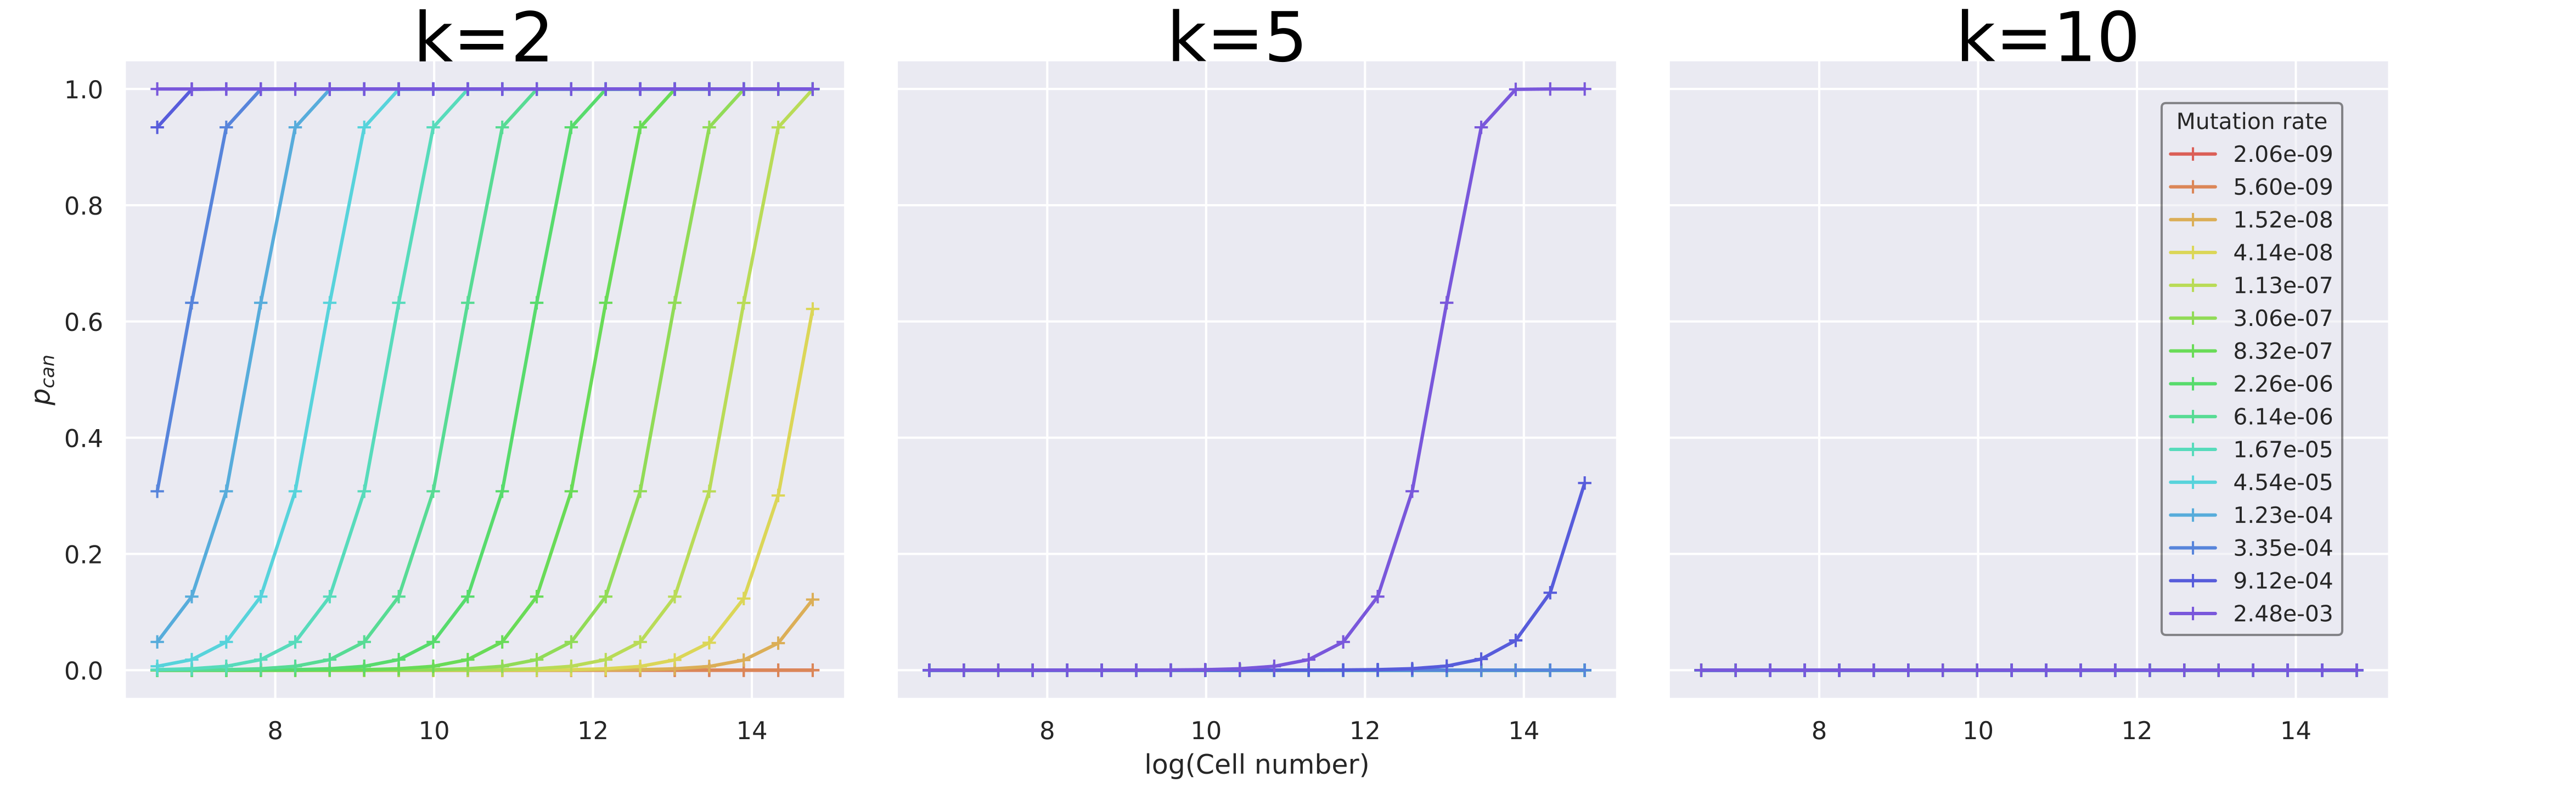
\includegraphics[width=\linewidth]{fig3.png}
			\caption{Incidence vs log($n$) for different $p$ and $k$}
		\end{figure}
		\end{minipage}

		\section{Selection models}
		\begin{minipage}{.5\linewidth}
		\begin{itemize}
			\item Linear evolution process, leading to mutation accumlation
			\item Discrere logistic equation for cell growth and competition, with one step growth making one day of lifespan
			\item Non-mutant growth rate, $g_{0}=0.007$, and a linear progression up to $g_{k}$ for the $k$th oncogenic mutation, at which cancer occurs
			\item $\Delta_{g}=\frac{g_{k}-g_{0}}{k}$ is randomized in the population for context-dependent selection, as N($\mu, \sigma$)
			\item $n \in [1.203*10^{6}, 2.649*10^{10}]$
			\item $p \in [3.775*10^{-11}, 3.059*10^{-7}]$
		\end{itemize}
		\end{minipage}
		\hspace{0.05\linewidth}
		\begin{minipage}{.45\linewidth}
			\begin{figure}[H]
				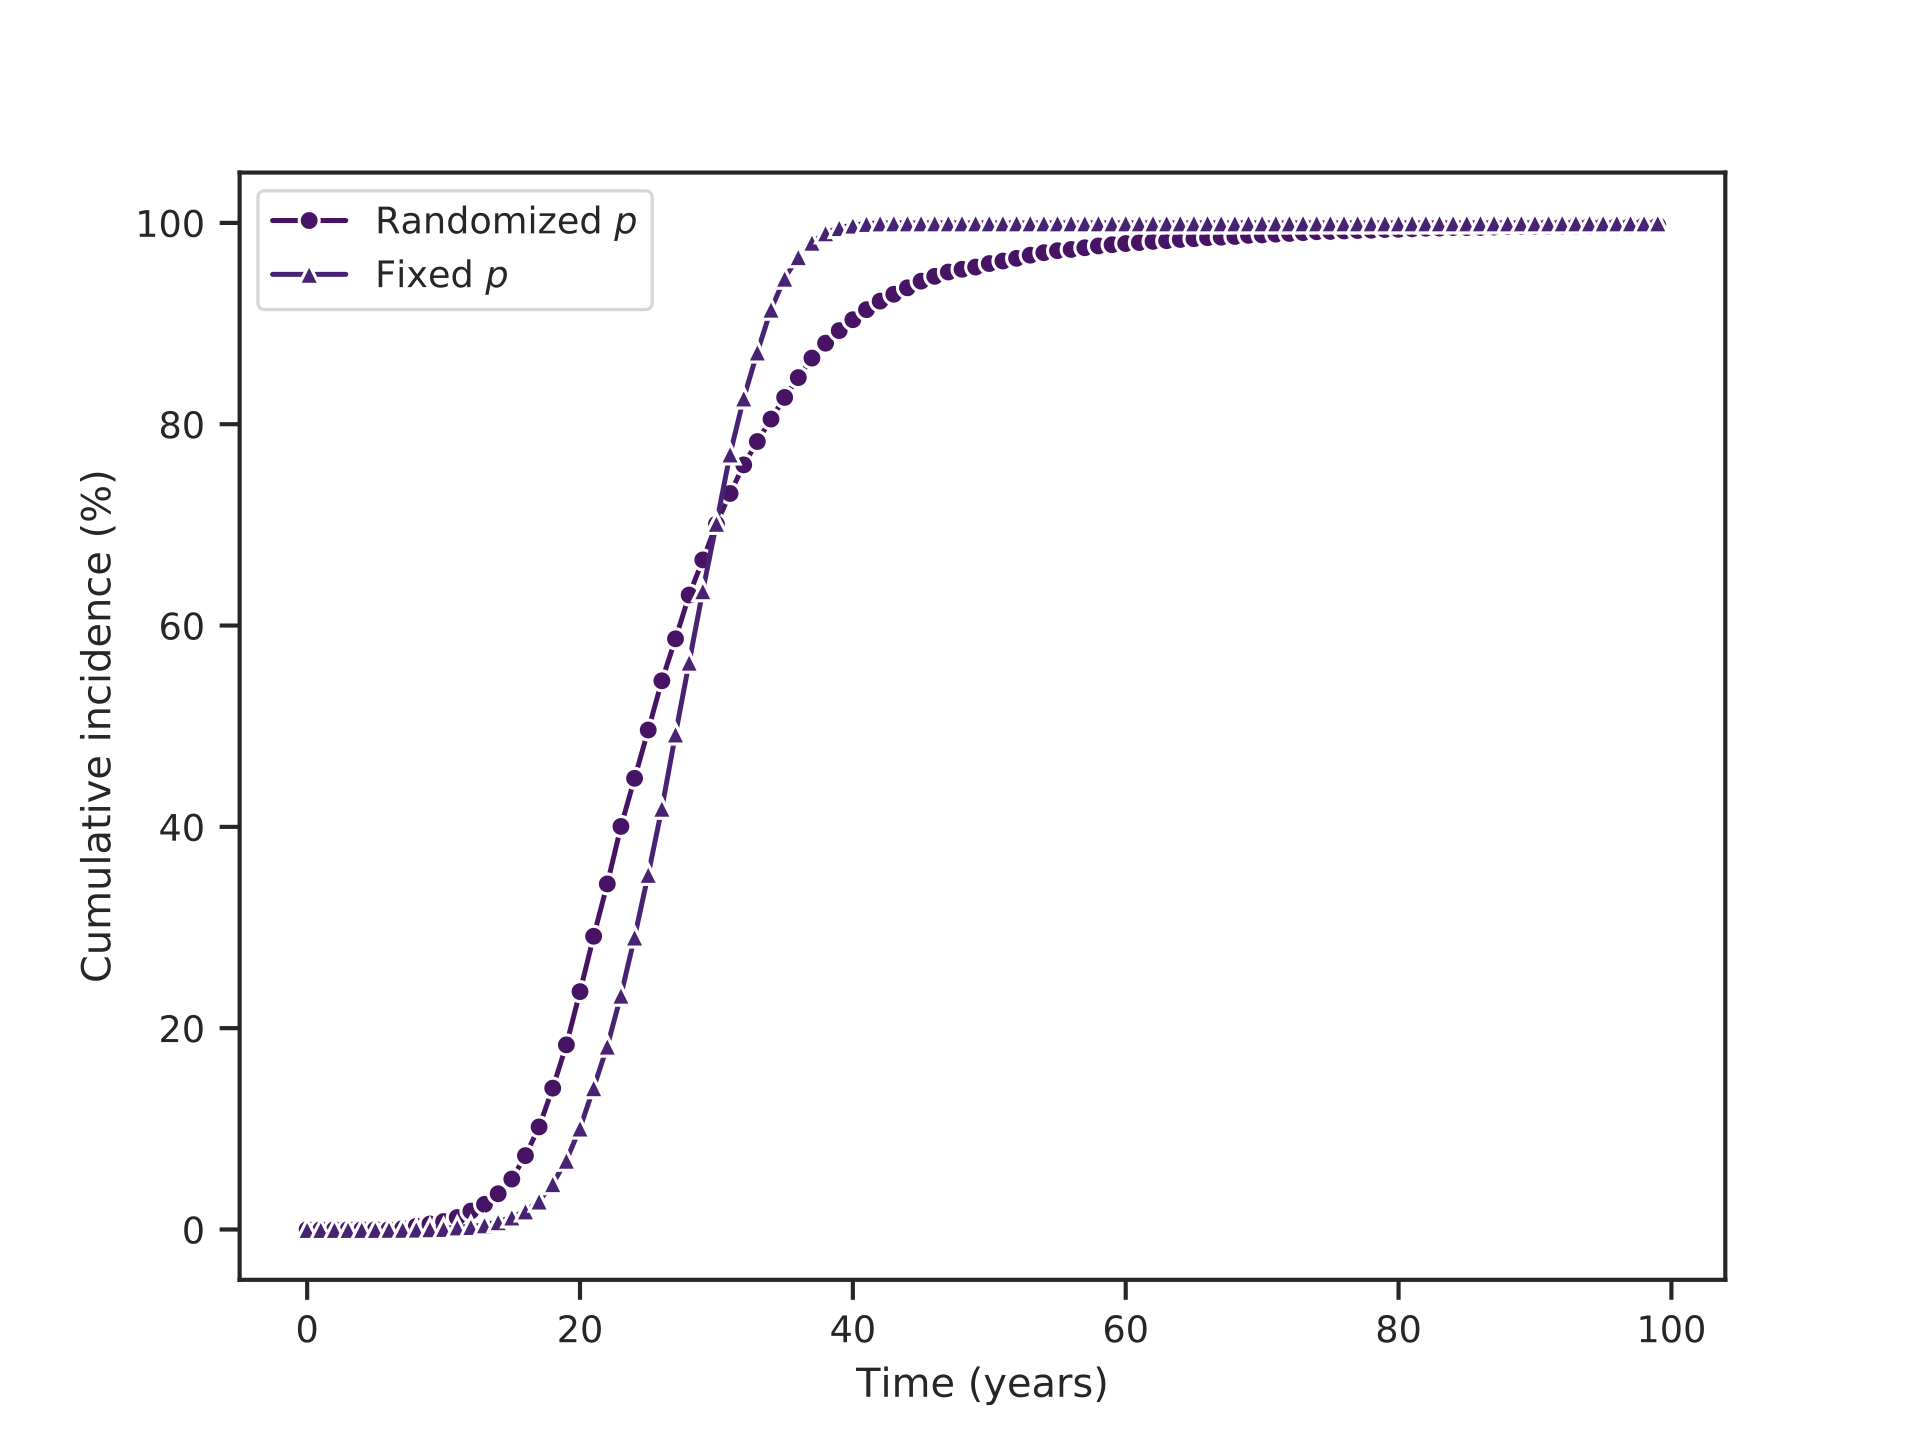
\includegraphics[width=\linewidth]{fig4.png}
				\caption{Context-independent model; randomized $p$ vs fixed $p$. Mean randomized $p \approx$ fixed $p$.}
			\end{figure}
		\end{minipage}

		\begin{flushleft}
			\begin{figure}[H]
				%			\def\svgwidth{0.2\columnwidth}
				%			\input{sat_pooled.pdf_tex}
				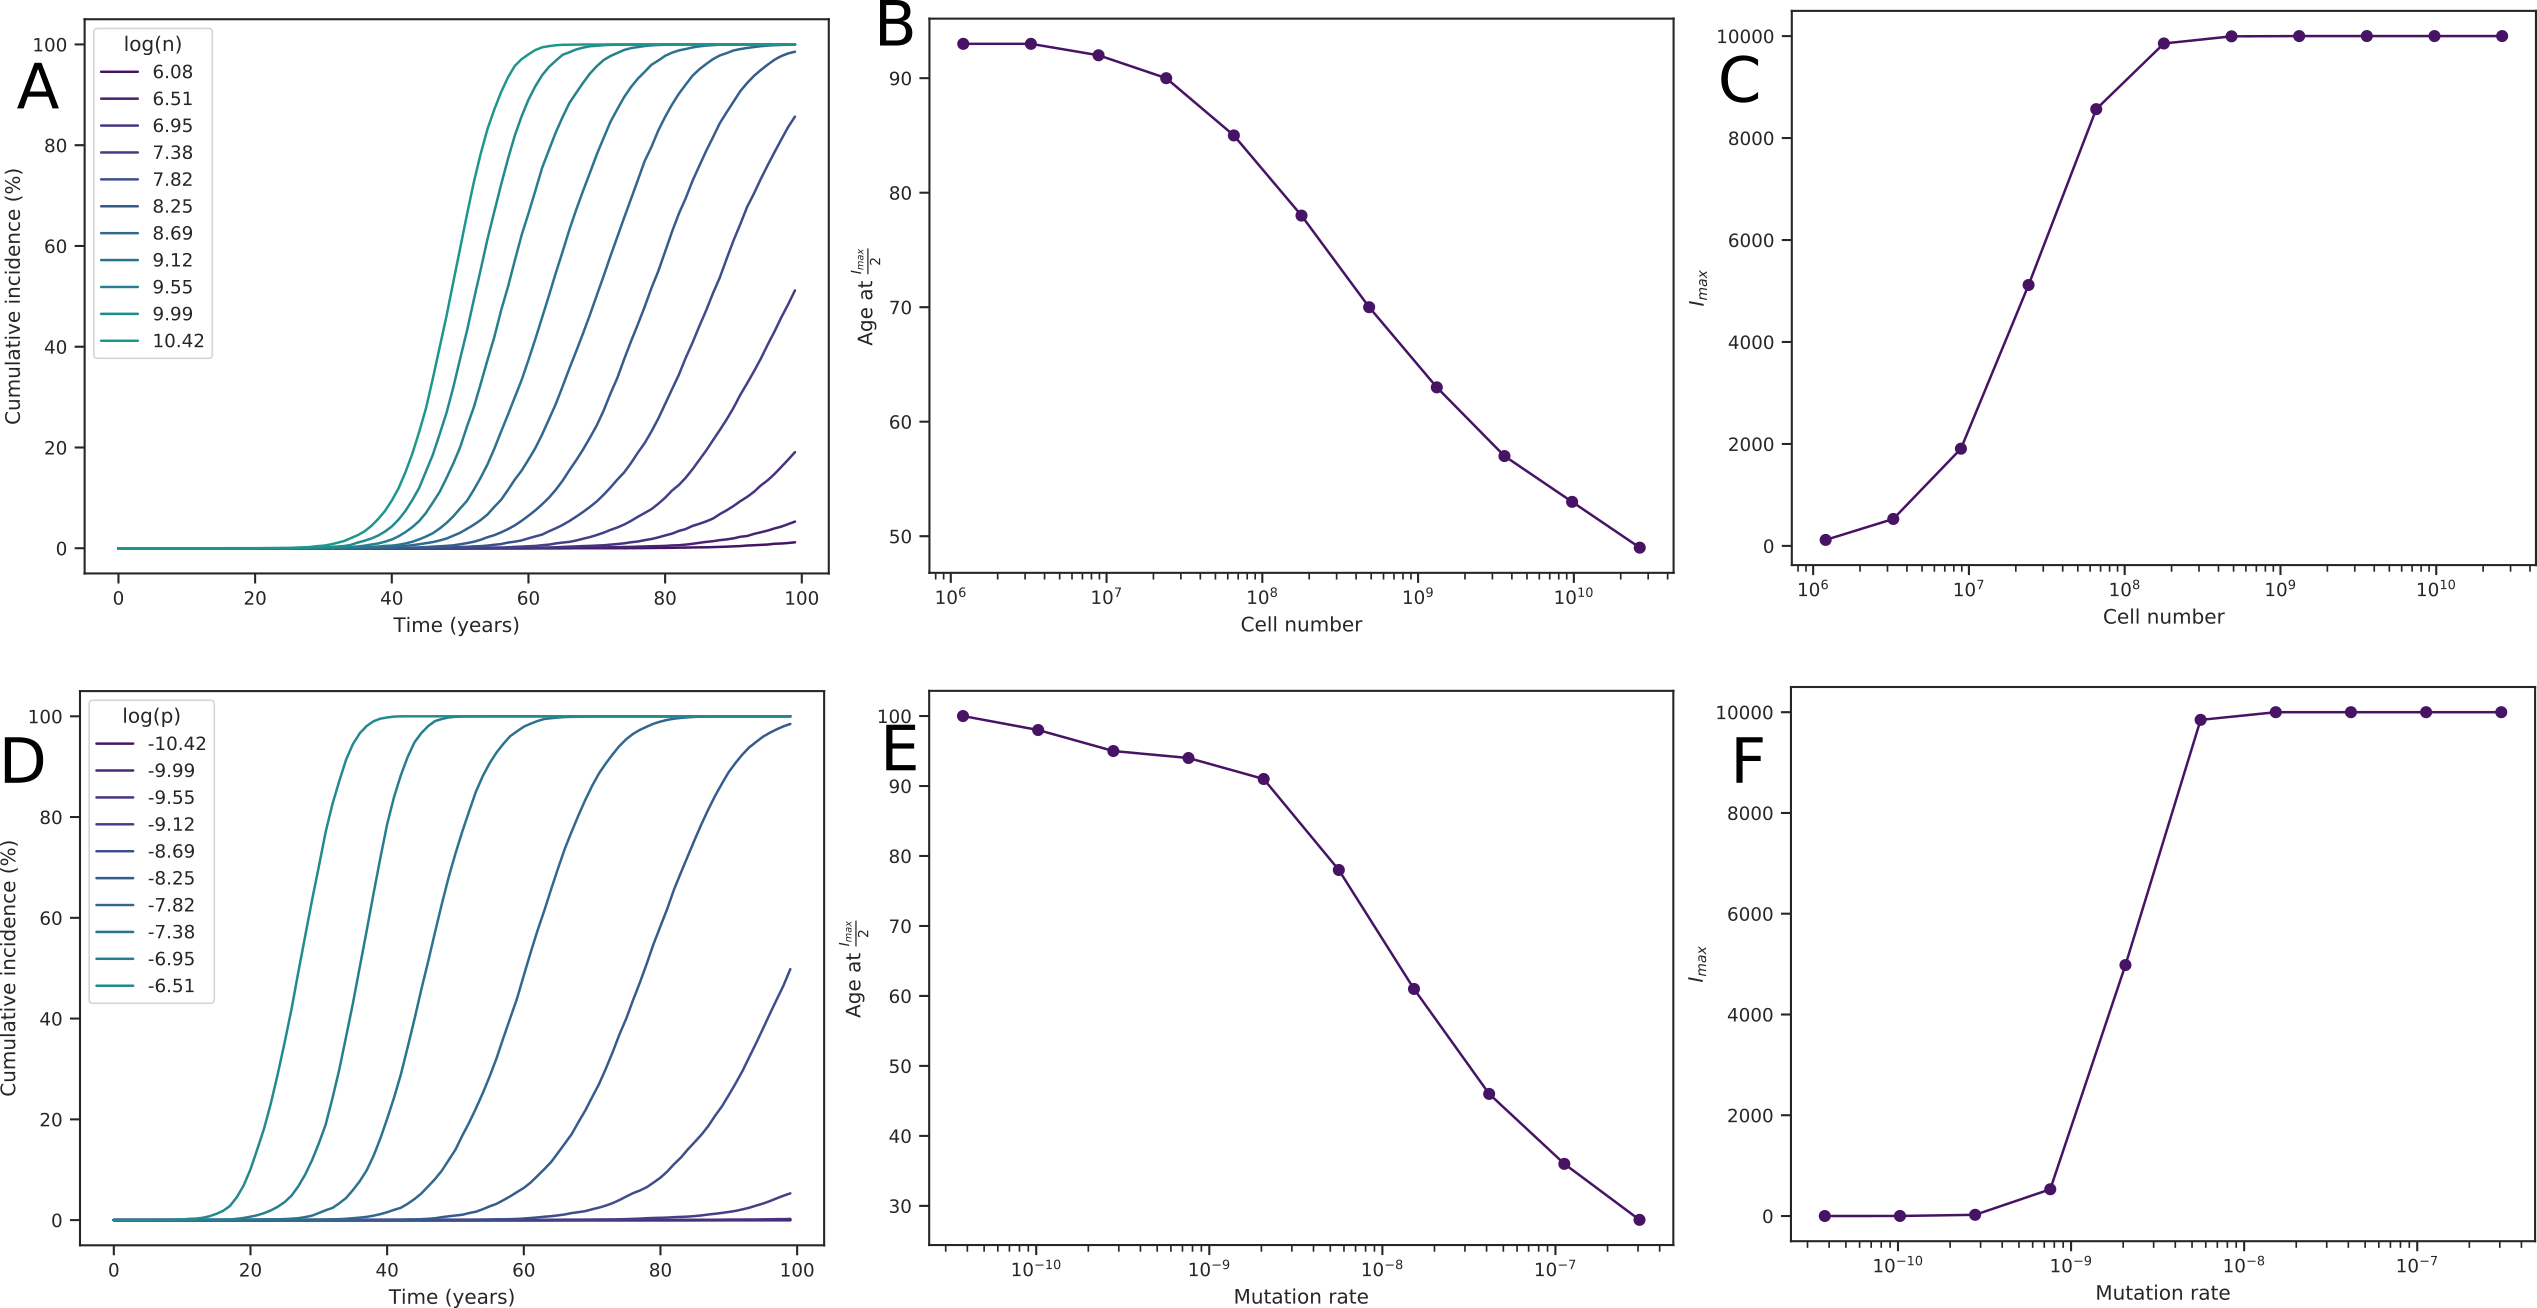
\includegraphics[width=\linewidth]{fig5.png}
				\caption{Context-independent selection; crude and cumulative incidence rates vs age, age at half maximum cumulative incidence, and maximum cumulative incidence, over the range of $n$ and $p$.}
			\end{figure}
			\begin{figure}[H]
				%			\def\svgwidth{0.2\columnwidth}
				%			\input{sat_pooled.pdf_tex}
				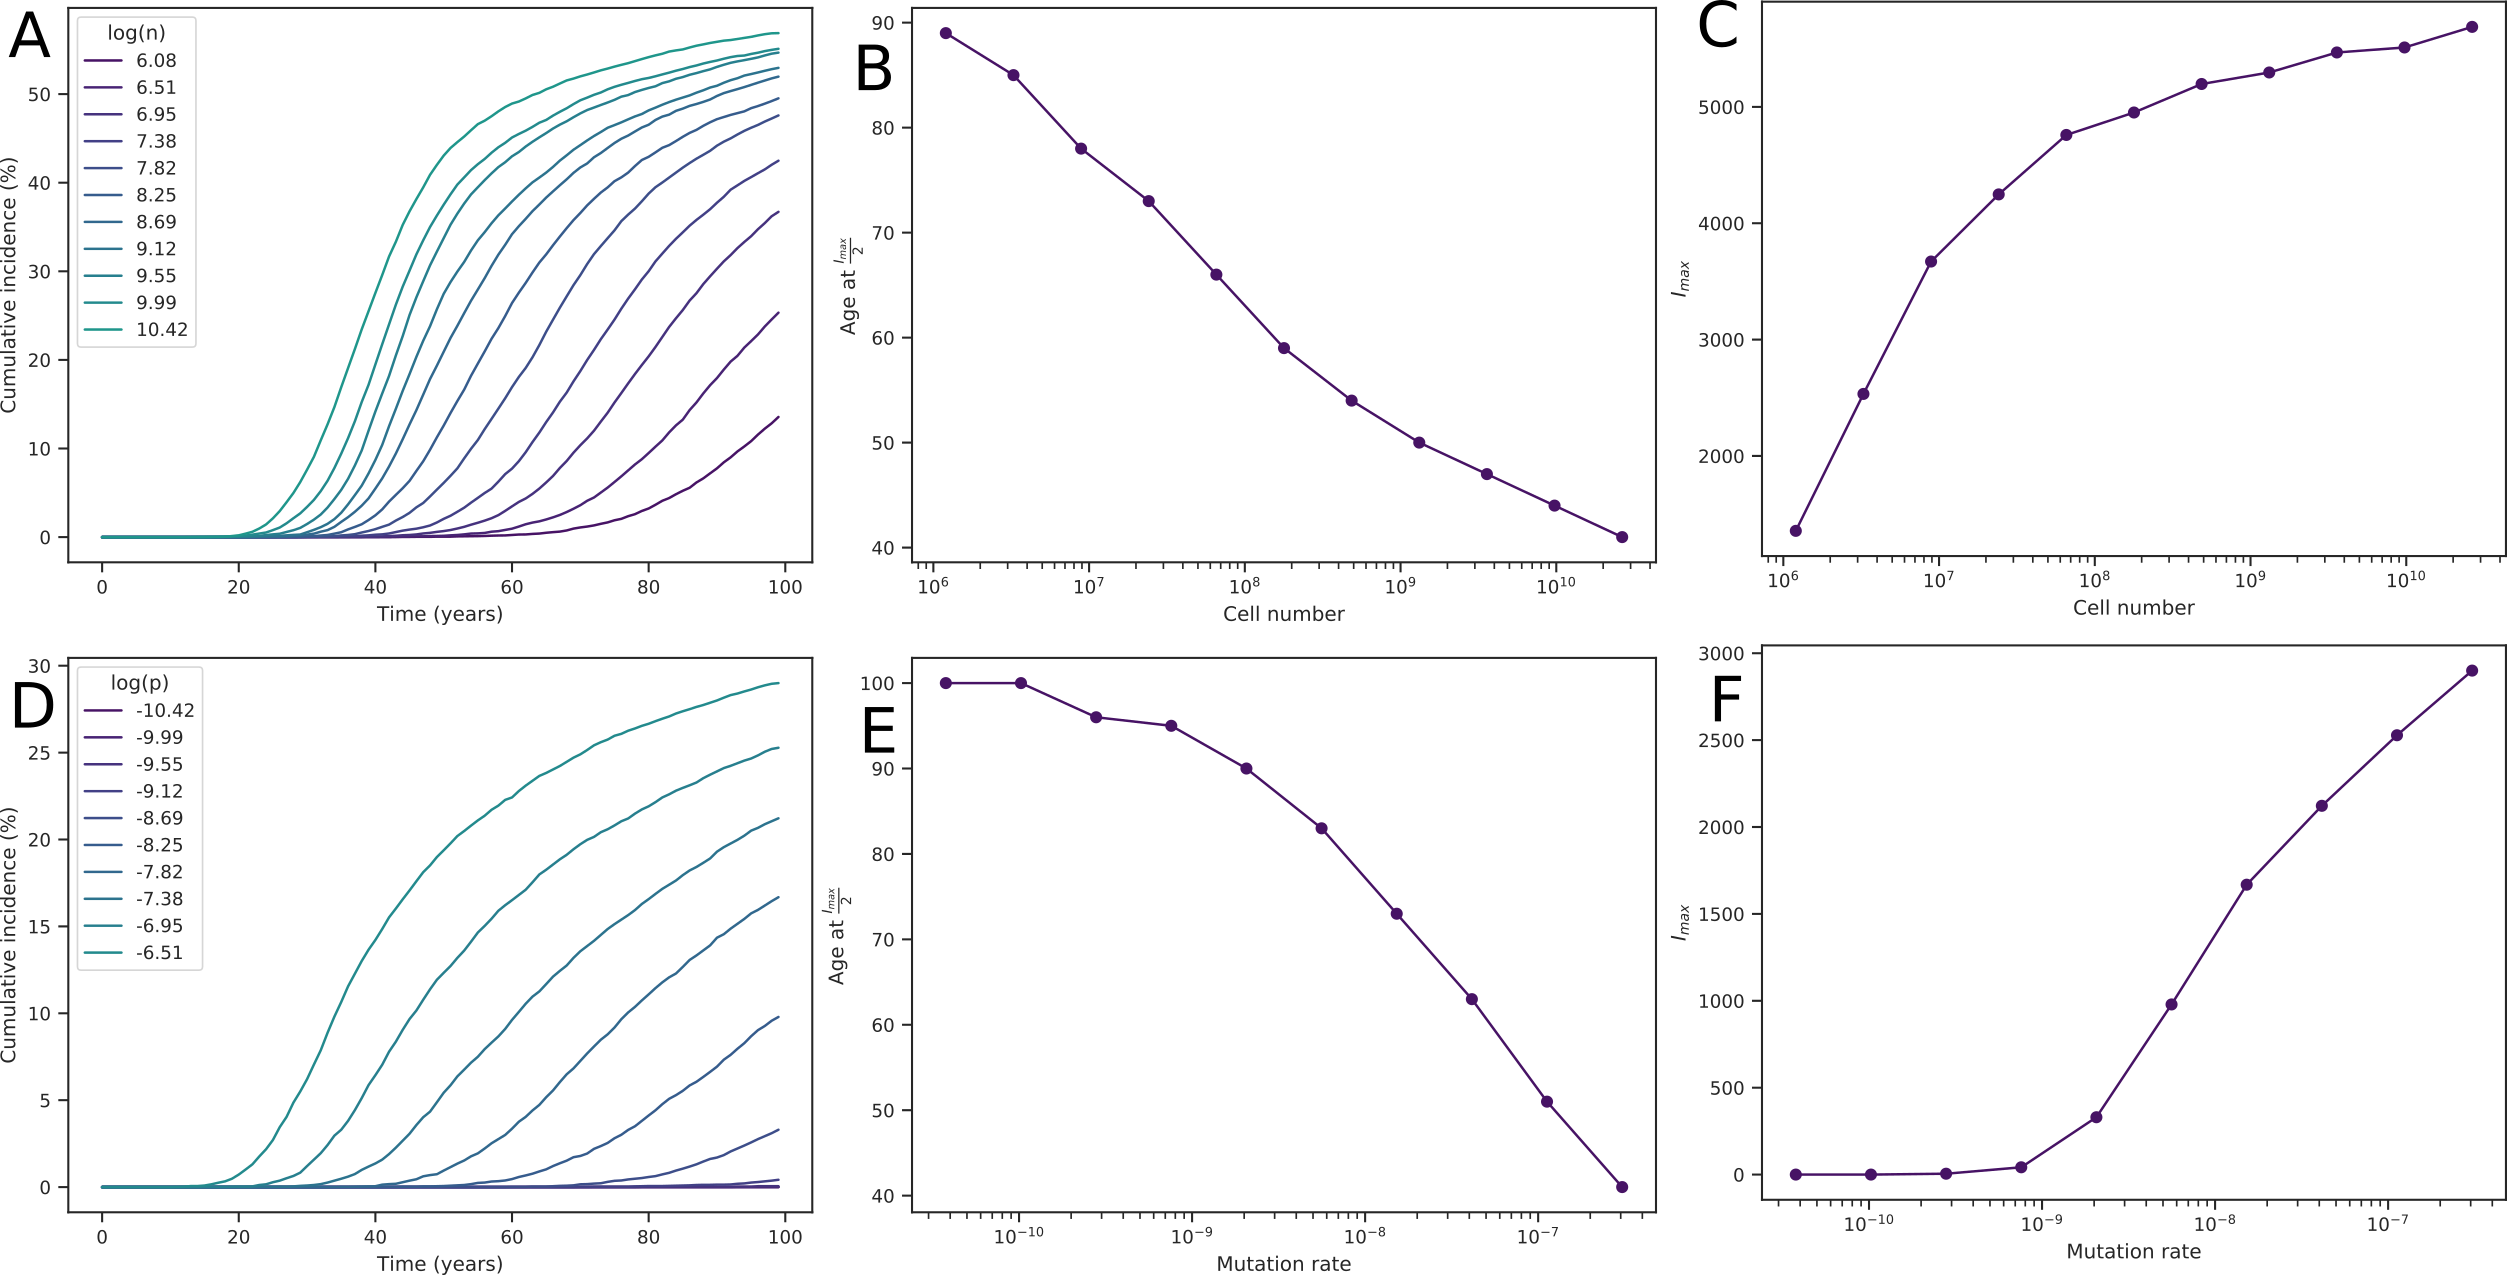
\includegraphics[width=\linewidth]{fig6.png}
				\caption{Same incidence parameters as above, for the context-dependent selection case.}
			\end{figure}
		\end{flushleft}
		
		\subsection{Effect of $k$}
		% \begin{minipage}{.5\linewidth}
			\begin{figure}[H]
			\centering
				%			\def\svgwidth{0.2\columnwidth}
				%			\input{higher_p.pdf_tex}
				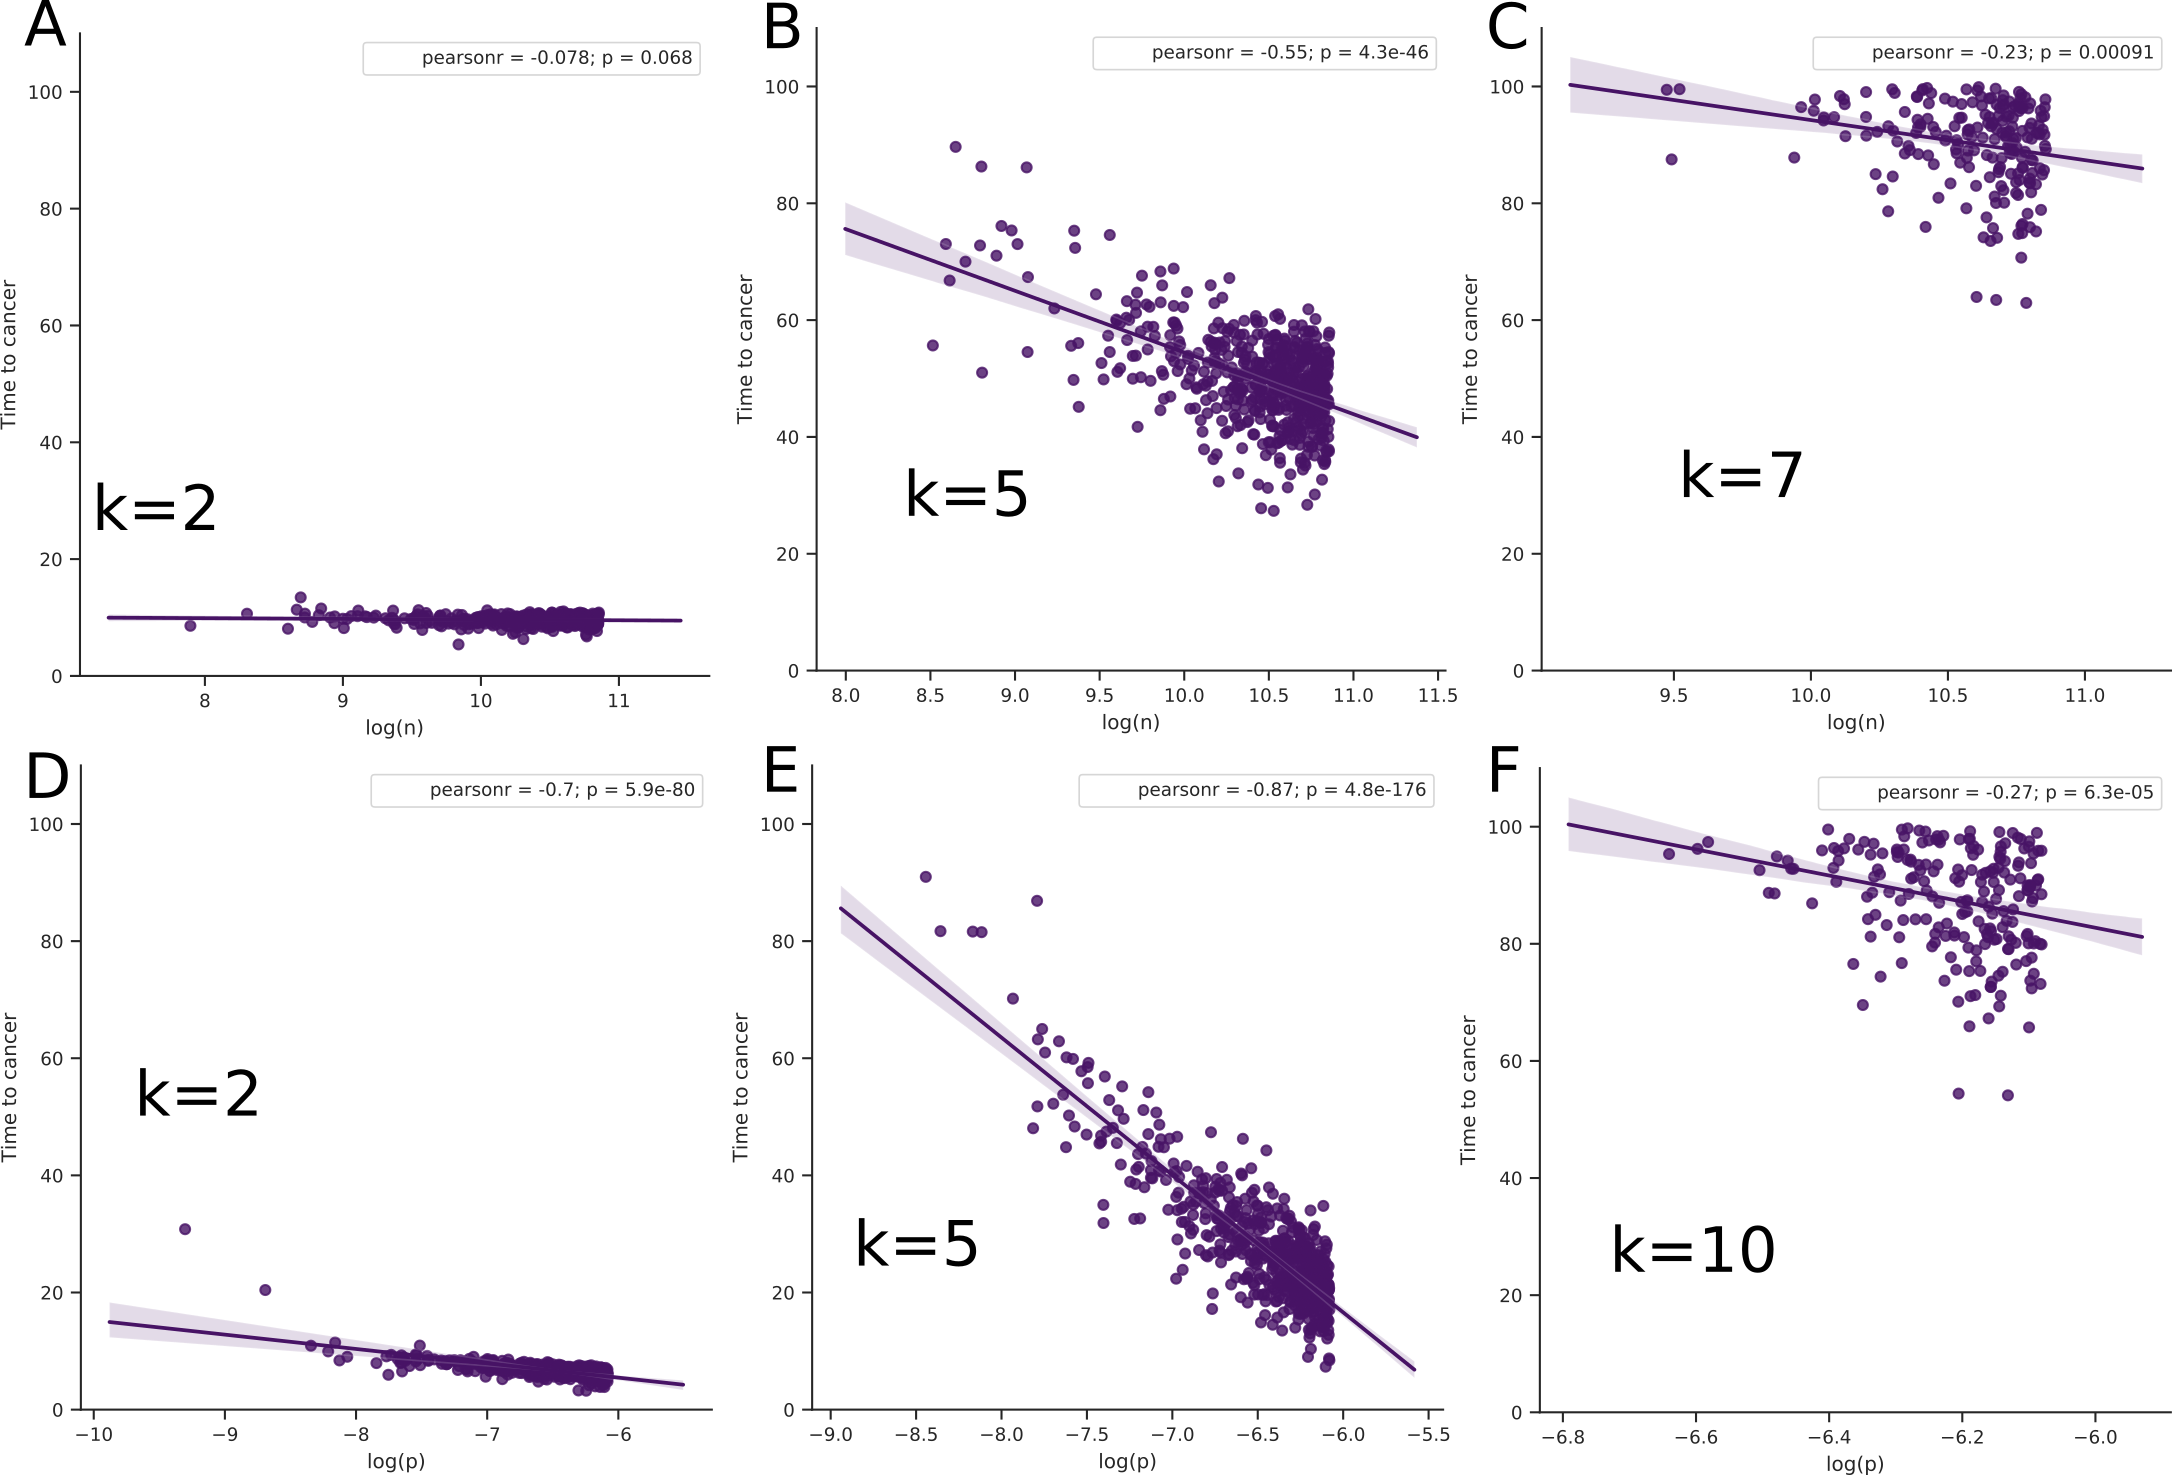
\includegraphics[width=.8\linewidth, height=.4\linewidth]{fig7.png}
				\caption{Context-independent selection case; association of time to cancer with $n$ and $p$ is modulated by $k$.}
			\end{figure}
		% \end{minipage}
			% \hspace{0.01\linewidth}
		% \begin{minipage}{.5\linewidth}
			\begin{figure}[H]
			\centering
				%			\def\svgwidth{0.2\columnwidth}
				%			\input{higher_p.pdf_tex}
				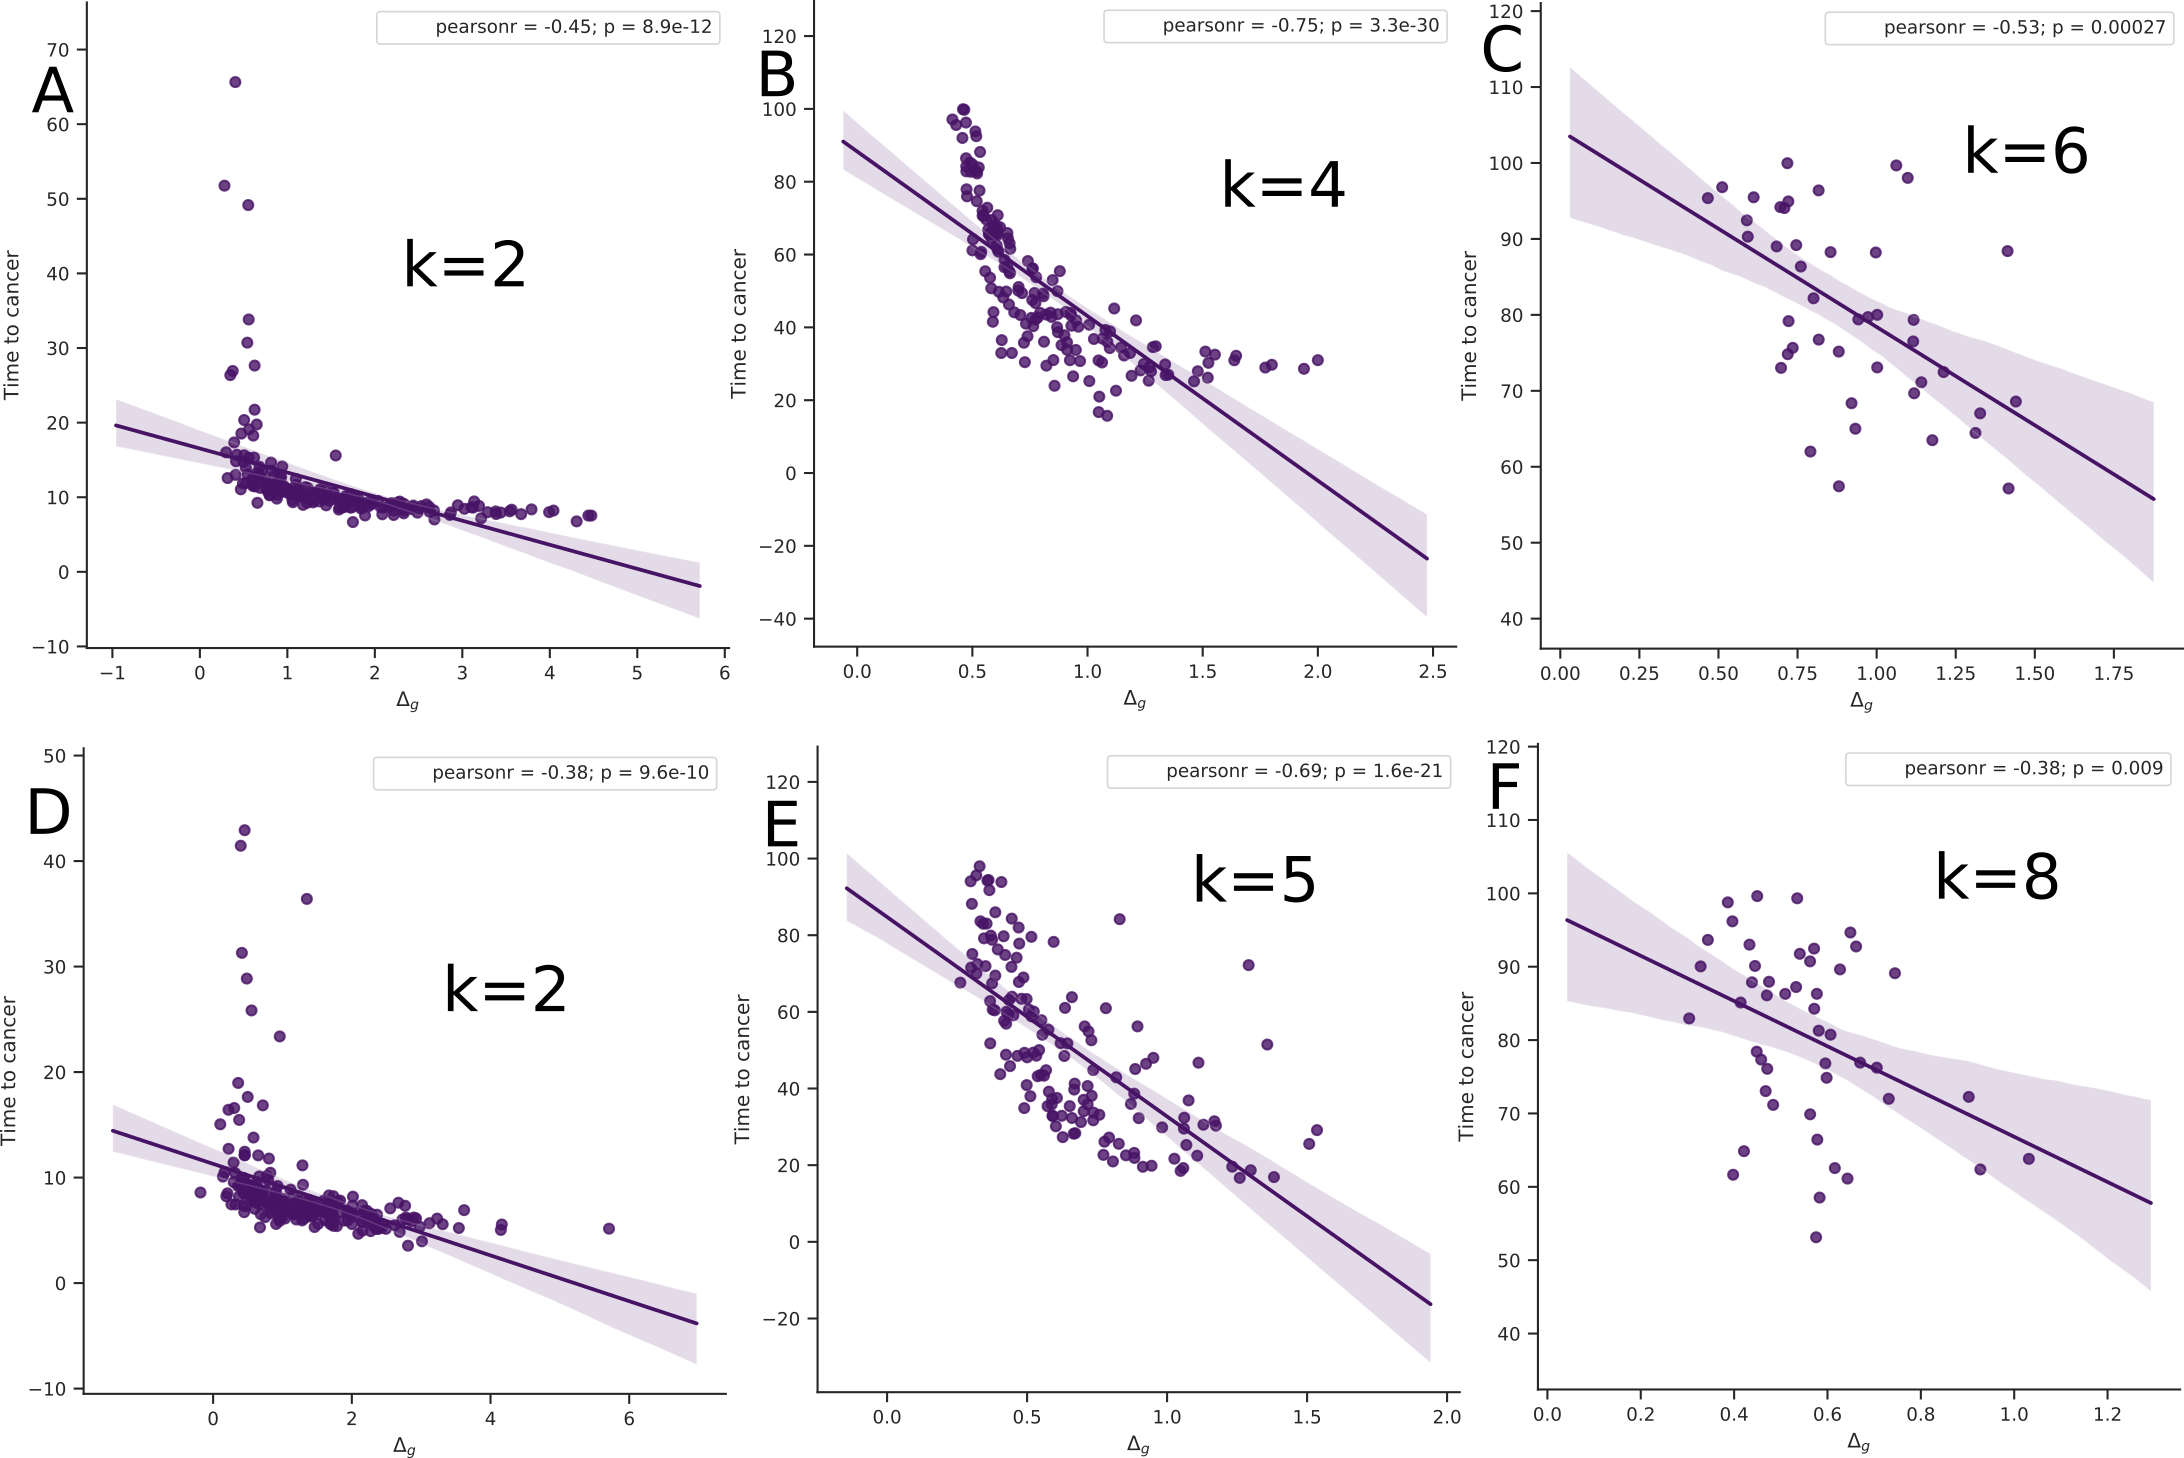
\includegraphics[width=.8\linewidth, height=.4\linewidth]{fig8.png}
				\caption{Context-dependent selection case; association of time to cancer with $\Delta_{g}$ is modulated by $k$.}
			\end{figure}
		% \end{minipage}

		\section{Conclusions}
		\begin{table}[H]
		\centering
			\begin{tabular}{p{.3\linewidth}|p{.2\linewidth}p{.25\linewidth}p{.225\linewidth}}
			\textbf{Epidemiological observation} & ``Bad luck'' & Context-independent selection & Context-dependent selection \\
			\hline
			\textbf{Total incidence < 30\%} & 100\% & 100\% & <100\% possible \\
			\textbf{Late-life decline} & No & No & Yes \\
			\textbf{Incidence vs $n$} & Threshold & Threshold & Progressive \\
			\textbf{Non-mutagenic carcinogens} & Incompatible & Incompatible & $g$ distribution \\
			\textbf{Peto's paradox} & Extrinsic\footnote[1]{Extrinsic explanations like evolved cancer defences are required.} & Extrinsic\footnote[1]{Extrinsic explanations like evolved cancer defences are required.} & Intrinsic \\
			\end{tabular}
		%\addtabletext{nomenclature for the TSs refers to the numbered species in the table.}
		\end{table}

		\begin{minipage}{.5\linewidth}
		\renewcommand*{\bibfont}{\small}
		\printbibliography
		\end{minipage}
		\hspace{0.01\linewidth}
		\begin{minipage}{.5\linewidth}
		\small
		\section*{Acknowledgements}
		The authors acknowledge support from IISER Pune, and valuable feedback from faculty members of the Department of Biology as well as the Watve Lab.
		\end{minipage}
	
	
	%--------------------------l--------------------------------------------------------------
	%	OBJECTIVES
	%----------------------------------------------------------------------------------------
	
	% DarkSlateGray color for the rest of the content
	
	%\section*{Main Objectives}
	%
	%\begin{enumerate}
	%\item Lorem ipsum dolor sit amet, consectetur.
	%\item Nullam at mi nisl. Vestibulum est purus, ultricies cursus volutpat sit amet, vestibulum eu.
	%\item Praesent tortor libero, vulputate quis elementum a, iaculis.
	%\item Phasellus a quam mauris, non varius mauris. Fusce tristique, enim tempor varius porta, elit purus commodo velit, pretium mattis ligula nisl nec ante.
	%\item Ut adipiscing accumsan sapien, sit amet pretium.
	%\item Estibulum est purus, ultricies cursus volutpat
	%\item Nullam at mi nisl. Vestibulum est purus, ultricies cursus volutpat sit amet, vestibulum eu.
	%\item Praesent tortor libero, vulputate quis elementum a, iaculis.
	%\end{enumerate}
	
	%----------------------------------------------------------------------------------------
	%	MATERIALS AND METHODS
	%----------------------------------------------------------------------------------------
	
	%\section*{Materials and Methods}
	%
	%Fusce magna risus, molestie ut porttitor in, consectetur sed mi. Vestibulum ante ipsum primis in faucibus orci luctus et ultrices posuere cubilia Curae; Pellentesque consectetur blandit pellentesque. Sed odio justo, viverra nec porttitor vel, lacinia a nunc. Suspendisse pulvinar euismod arcu, sit amet accumsan enim fermentum quis. In id mauris ut dui feugiat egestas. Vestibulum ac turpis lacinia nisl commodo sagittis eget sit amet sapien.
	%
	%%------------------------------------------------
	%
	%\subsection*{Mathematical Section}
	%
	%Nulla vel nisl sed mauris auctor mollis non sed. 
	%
	%\begin{equation}
	%E = mc^{2}
	%\label{eqn:Einstein}
	%\end{equation}
	%
	%Curabitur mi sem, pulvinar quis aliquam rutrum. (1) edf (2)
	%, $\Omega=[-1,1]^3$, maecenas leo est, ornare at. $z=-1$ edf $z=1$ sed interdum felis dapibus sem. $x$ set $y$ ytruem. 
	%Turpis $j$ amet accumsan enim $y$-lacina; 
	%ref $k$-viverra nec porttitor $x$-lacina. 
	%
	%Vestibulum ac diam a odio tempus congue. Vivamus id enim nisi:
	%
	%\begin{eqnarray}
	%\cos\bar{\phi}_k Q_{j,k+1,t} + Q_{j,k+1,x}+\frac{\sin^2\bar{\phi}_k}{T\cos\bar{\phi}_k} Q_{j,k+1} &=&\nonumber\\ 
	%-\cos\phi_k Q_{j,k,t} + Q_{j,k,x}-\frac{\sin^2\phi_k}{T\cos\phi_k} Q_{j,k}\label{edgek}
	%\end{eqnarray}
	%and
	%\begin{eqnarray}
	%\cos\bar{\phi}_j Q_{j+1,k,t} + Q_{j+1,k,y}+\frac{\sin^2\bar{\phi}_j}{T\cos\bar{\phi}_j} Q_{j+1,k}&=&\nonumber \\
	%-\cos\phi_j Q_{j,k,t} + Q_{j,k,y}-\frac{\sin^2\phi_j}{T\cos\phi_j} Q_{j,k}.\label{edgej}
	%\end{eqnarray} 
	%
	%Nulla sed arcu arcu. Duis et ante gravida orci venenatis tincidunt. Fusce vitae lacinia metus. Pellentesque habitant morbi. $\mathbf{A}\underline{\xi}=\underline{\beta}$ Vim $\underline{\xi}$ enum nidi $3(P+2)^{2}$ lacina. Id feugain $\mathbf{A}$ nun quis; magno.
	%
	%%----------------------------------------------------------------------------------------
	%%	RESULTS 
	%%----------------------------------------------------------------------------------------
	%
	%\section*{Results}
	%
	%Donec faucibus purus at tortor egestas eu fermentum dolor facilisis. Maecenas tempor dui eu neque fringilla rutrum. Mauris \emph{lobortis} nisl accumsan. Aenean vitae risus ante.
	%%
	%\begin{wraptable}{l}{12cm} % Left or right alignment is specified in the first bracket, the width of the table is in the second
	%\begin{tabular}{l l l}
	%\toprule
	%\textbf{Treatments} & \textbf{Response 1} & \textbf{Response 2}\\
	%\midrule
	%Treatment 1 & 0.0003262 & 0.562 \\
	%Treatment 2 & 0.0015681 & 0.910 \\
	%Treatment 3 & 0.0009271 & 0.296 \\
	%\bottomrule
	%\end{tabular}
	%\captionof{table}{\color{Green} Table caption}
	%\end{wraptable}
	%%
	%Phasellus imperdiet, tortor vitae congue bibendum, felis enim sagittis lorem, et volutpat ante orci sagittis mi. Morbi rutrum laoreet semper. Morbi accumsan enim nec tortor consectetur non commodo nisi sollicitudin. Proin sollicitudin. Pellentesque eget orci eros. Fusce ultricies, tellus et pellentesque fringilla, ante massa luctus libero, quis tristique purus urna nec nibh.
	%
	%Nulla ut porttitor enim. Suspendisse venenatis dui eget eros gravida tempor. Mauris feugiat elit et augue placerat ultrices. Morbi accumsan enim nec tortor consectetur non commodo. Pellentesque condimentum dui. Etiam sagittis purus non tellus tempor volutpat. Donec et dui non massa tristique adipiscing. Quisque vestibulum eros eu. Phasellus imperdiet, tortor vitae congue bibendum, felis enim sagittis lorem, et volutpat ante orci sagittis mi. Morbi rutrum laoreet semper. Morbi accumsan enim nec tortor consectetur non commodo nisi sollicitudin.
	%
	%\begin{center}\vspace{1cm}
	%\includegraphics[width=0.8\linewidth]{placeholder}
	%\captionof{figure}{\color{Green} Figure caption}
	%\end{center}\vspace{1cm}
	%
	%In hac habitasse platea dictumst. Etiam placerat, risus ac.
	%
	%Adipiscing lectus in magna blandit:
	%
	%\begin{center}\vspace{1cm}
	%\begin{tabular}{l l l l}
	%\toprule
	%\textbf{Treatments} & \textbf{Response 1} & \textbf{Response 2} \\
	%\midrule
	%Treatment 1 & 0.0003262 & 0.562 \\
	%Treatment 2 & 0.0015681 & 0.910 \\
	%Treatment 3 & 0.0009271 & 0.296 \\
	%\bottomrule
	%\end{tabular}
	%\captionof{table}{\color{Green} Table caption}
	%\end{center}\vspace{1cm}
	%
	%Vivamus sed nibh ac metus tristique tristique a vitae ante. Sed lobortis mi ut arcu fringilla et adipiscing ligula rutrum. Aenean turpis velit, placerat eget tincidunt nec, ornare in nisl. In placerat.
	%
	%\begin{center}\vspace{1cm}
	%\includegraphics[width=0.8\linewidth]{placeholder}
	%\captionof{figure}{\color{Green} Figure caption}
	%\end{center}\vspace{1cm}
	%
	%%----------------------------------------------------------------------------------------
	%%	CONCLUSIONS
	%%----------------------------------------------------------------------------------------
	%
	%\color{SaddleBrown} % SaddleBrown color for the conclusions to make them stand out
	%
	%\section*{Conclusions}
	%
	%\begin{itemize}
	%\item Pellentesque eget orci eros. Fusce ultricies, tellus et pellentesque fringilla, ante massa luctus libero, quis tristique purus urna nec nibh. Phasellus fermentum rutrum elementum. Nam quis justo lectus.
	%\item Vestibulum sem ante, hendrerit a gravida ac, blandit quis magna.
	%\item Donec sem metus, facilisis at condimentum eget, vehicula ut massa. Morbi consequat, diam sed convallis tincidunt, arcu nunc.
	%\item Nunc at convallis urna. isus ante. Pellentesque condimentum dui. Etiam sagittis purus non tellus tempor volutpat. Donec et dui non massa tristique adipiscing.
	%\end{itemize}
	%
	%\color{DarkSlateGray} % Set the color back to DarkSlateGray for the rest of the content
	%
	
	%\section*{Acknowledgements}
	%
	%Etiam fermentum, arcu ut gravida fringilla, dolor arcu laoreet justo, ut imperdiet urna arcu a arcu. Donec nec ante a dui tempus consectetur. Cras nisi turpis, dapibus sit amet mattis sed, laoreet.
	
	%----------------------------------------------------------------------------------------
	
\end{multicols}
\end{document}